\documentclass[final,hyperref={pdfpagelabels=false},xcolor=table]{beamer}
\mode<presentation>{
	\usetheme{ucb}
}
\usepackage[size=custom,width=101.6,height=76.2,scale=1.5]{beamerposter}
\usepackage{multicol}
\usepackage{graphicx}
\usepackage{textcomp}
\usepackage{pbox}
%\usepackage{booktabs}
%\usepackage{multirow}
%\usepackage{listings}
\usepackage{siunitx}
\usepackage{blindtext}

\definecolor{ucb-pacific}{HTML}{5B6770}

\newcommand{\uT}{{\textmu}T}
\setlength{\leftmargini}{4em}

\title{Hardware Acceleration of Key-Value Stores}
\author{Sagar Karandikar, Howard Mao, Albert Ou, Soumya Basu}
\advisor{Krste Asanovi\'{c}}
\institute[UC Berkeley]{\textsc{University of California, Berkeley}}
\date[2014-12-11]{CS262a, 11 December 2014}

\begin{document}
\begin{frame}
\vspace{-1.5em}
\begin{columns}[t]
	\begin{column}{0.3\linewidth}
	\begin{block}{Motivation}
    \begin{itemize}
        \item In datacenter applications, path through CPU/Kernel/Application accounts for 86\% of total request latency
        \item Goal: Use hardware accelerator to serve popular requests for a key-value store, eliminate the CPU path in common case
        \item Many workloads have an access pattern suitable for a small cache
            \begin{itemize}
                \item A study conducted by Facebook on their memcached workload
                    showed that 10\% of the keys accounted for 90\% of the
                    requests.
                \item The study also showed that most values were relatively
                    small, about 1 kB.
            \end{itemize}

    \end{itemize}
%In Memcached in cluster mode, the software stack of the end host takes about
%86-95 percent of the total latency. A large part of that latency comes from the
%fact that we have to interrupt the CPU on every packet that it processes. Our
%insight is that by servicing hot requests on an FPGA instead of in software, we
%can substantially reduce the latency for most requests.

\end{block}

\vspace{1ex}

\begin{block}{Related Work}
\begin{itemize}
    \item A 2013 paper by Lim et al. proposed a system dubbed
        "Thin Servers with Smart Pipes", which served memcached get requests
        from FPGA hardware.
    \item However, the FPGA hardware handled get requests by accessing DRAM,
        not a local SRAM cache.
\end{itemize}

\end{block}

    \vspace{1ex}
    \begin{block}{Infrastructure and System Design}
    \begin{itemize}
        \item Node(s): Xilinx ZC706 FPGA Evaluation Platform
            \begin{itemize}
                \item RISC-V Rocket Core @ 50MHz
                    \begin{itemize}
                        \item Single Issue, In-order, 6-stage pipeline
                        \item ASIC version most nearly comparable with ARM Cortex-A5
                    \end{itemize}
                \item 512 MiB DRAM
                \item Brocade 1GE Copper SFP Transceiver
                    \begin{itemize}
                        \item Xilinx Tri-Mode Ethernet MAC
                        \item Xilinx 1000Base-X PCS/PMA
                    \end{itemize}

            \end{itemize} 
        \item Infrastructure Milestones
            \begin{itemize}
                \item No pre-existing hardware devices for Rocket Core
                \item Built first RISC-V hardware device: register-mapped NIC
                    \begin{itemize}
                        \item First \texttt{telnet/ssh} into a physical RISC-V machine
                    \end{itemize}
                \item Evolved to DMA-based NIC for performance
            \end{itemize}
    \end{itemize}

    %INSERT BOARD PIC HERE
\begin{multicols}{2}
    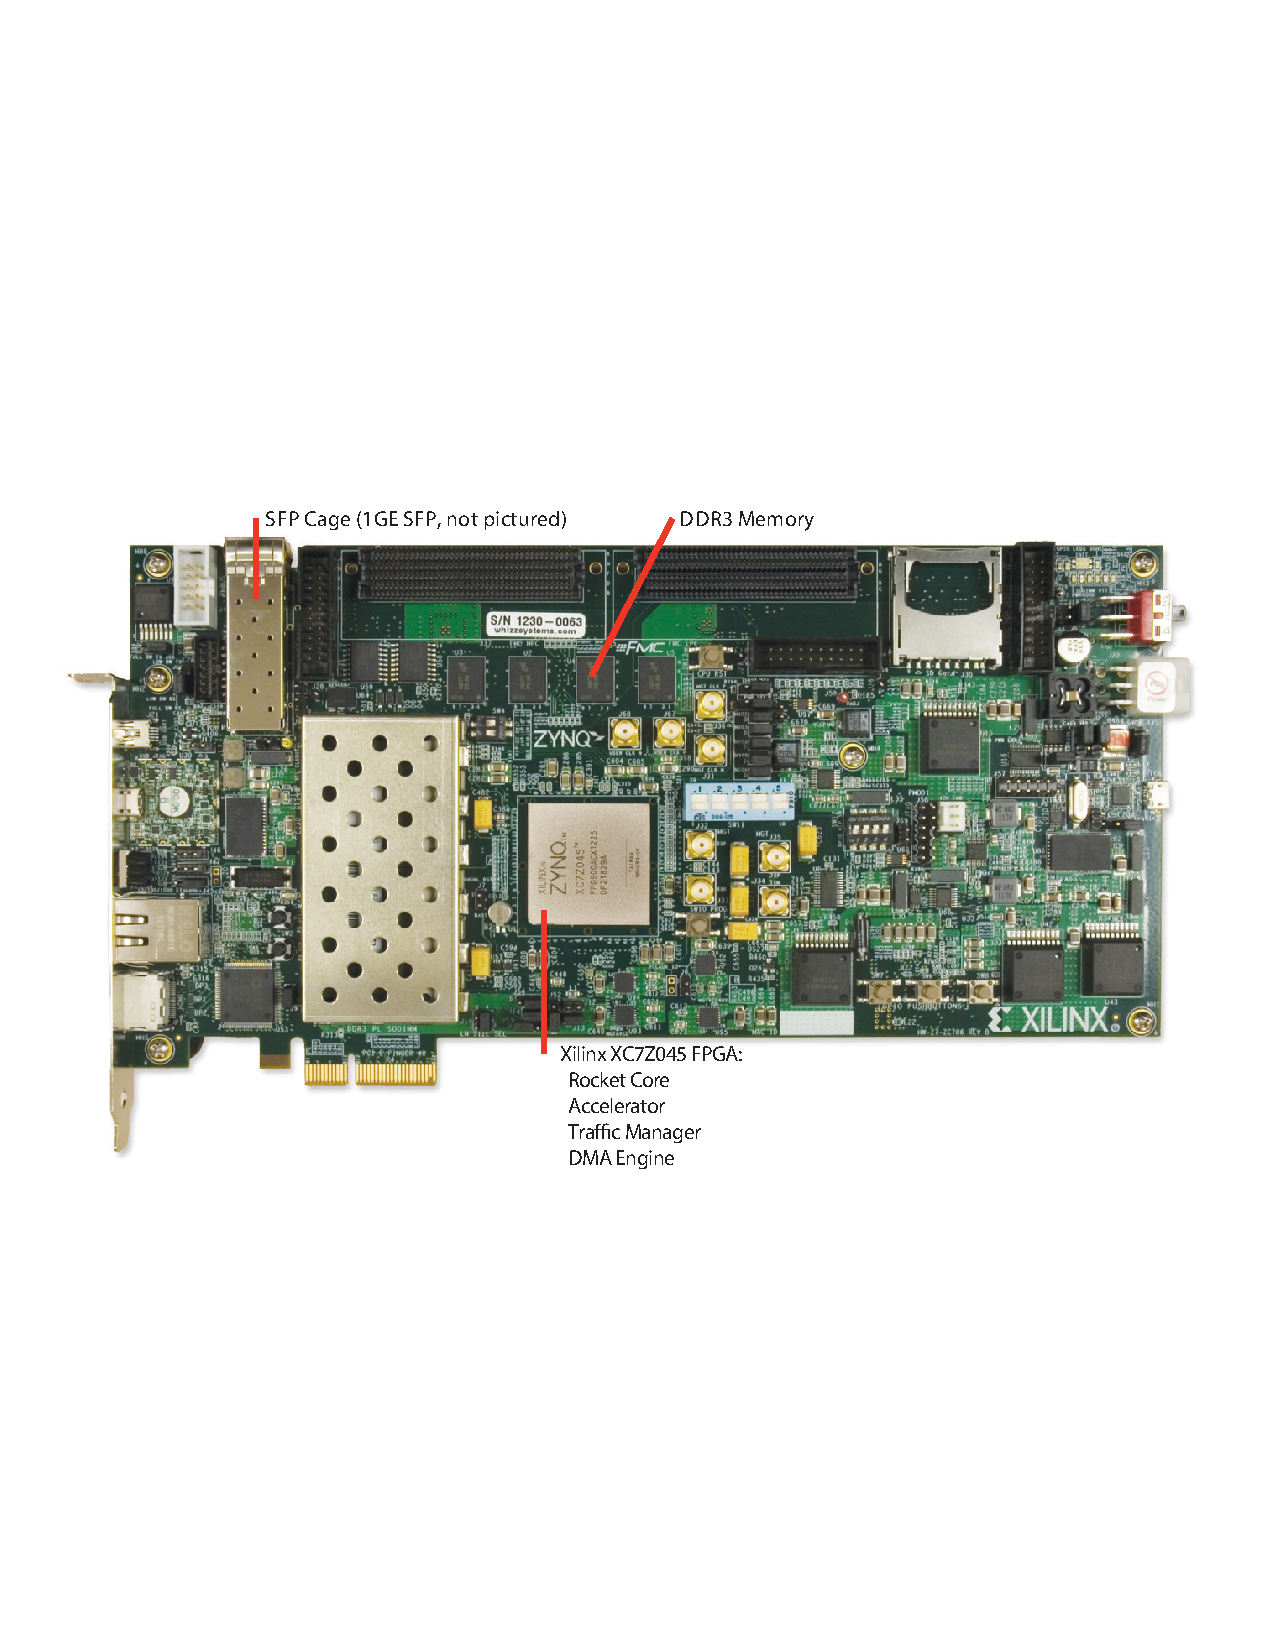
\includegraphics[width=\linewidth]{img/zc706.pdf}
\columnbreak
    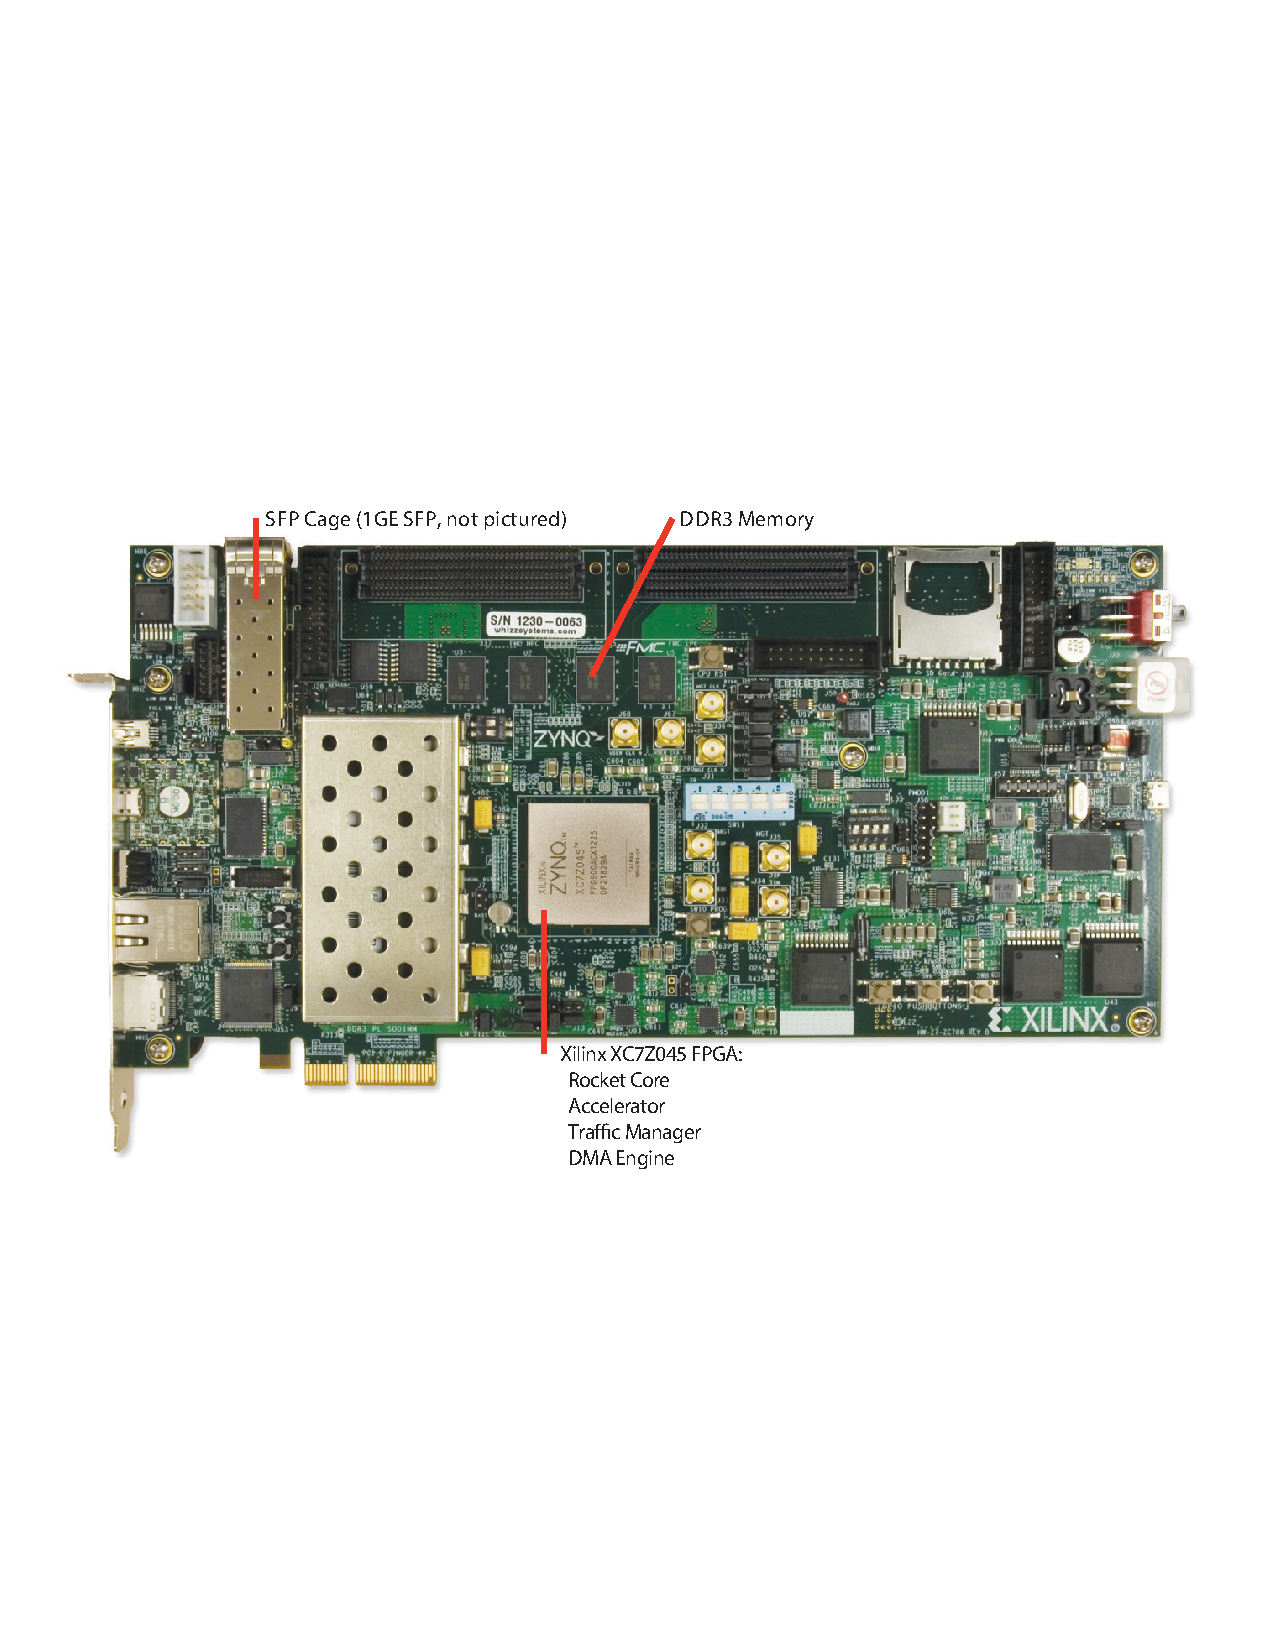
\includegraphics[width=\linewidth]{img/zc706.pdf}
\end{multicols}

\end{block}



	\end{column}

	\begin{column}{0.3\linewidth}
    \begin{block}{Hardware}
* Changes to the system go here [Block diagrams and stuff]
* Talk a little about the accelerator and filter.
\end{block}

    \vspace{1ex}
    \begin{block}{Software}
\begin{itemize}
\footnotesize
\item Manages what keys and values are stored on the accelerator
\item Controls the accelerator through the RoCC co-processor interface, which
	provides custom instructions for setting keys and values
\item Responsible for implementing cache replacement policies
	\begin{itemize}
	\footnotesize
	\item Identification of the most popular keys as candidates for offloading
	\item Invalidation of stale entries
	\end{itemize}
\end{itemize}

%Another part of the software is when to push each key to the accelerator. For
%this, we approximated how memcached is used in cluster mode where every key is
%pushed to the cache. However, interrupting the accelerator to push every key is
%very expensive and most of the keys are part of the long tail of our input
%distribution. Thus, we probabilistically insert keys to the accelerator, so hot
%keys are likely to get in while keys in the tail aren't very likely to get
%pushed.

\end{block}

	\end{column}

	\begin{column}{0.3\linewidth}
    \begin{block}{Floorplan}
*Insert floorplan diagram here



Without Accelerator / Traffic Manager
-------------------------------------


Utilization

\begin{center}
\begin{tabular}{ | c | c | c | c | c |} \hline
    Resource        & \pbox{20cm}{Utilization \\ (w/o A+TM)} & \pbox{20cm}{Utilization \\ (w/A+TM)} & Available \\ \hline
Slice LUTs      & 37358 (17.09\%)        &                & 218600    \\  \hline
Slice Registers & 27024 (6.18\%)         &                & 437200    \\  \hline
Memory          & 118   (21.65\%)        &                & 545       \\  \hline
DSP             & 15    (1.67\%)         &                & 900       \\  \hline
IO              & 15    (3.38\%)         &                & 444       \\  \hline
GT Channels     & 1     (6.25\%)         &                & 16        \\  \hline
Clocking        & 6     (18.75\%)        &                & 32        \\  \hline

\end{tabular}
\end{center}




\end{block}

    \vspace{1ex}
    \begin{block}{Preliminary Evaluation}
    \includegraphics[width=\linewidth]{img/graph.png}
    
    %* Insert latency graph here.
%* Insert throughput graph here.
%
%Extrapolate to cluster mode (talk about speedup of cluster mode). Use the 86
%percent pessimestic approximation to Amdahl's law.

\end{block}

    \vspace{1ex}
    \section{Conclusion}

In this paper, we design a hardware accelerator for the Memcached key-value
store and evaluate it on the ZC706 FPGA development board. By storing keys and
values in a dedicated SRAM cache and serving responses directly to the NIC 
without involving the CPU, our accelerator delivers an order of magnitude
improvement in latency. We furthermore show that our accelerator can store
enough key-value pairs to serve 40\% of requests in a real-world workload.

	\end{column}
\end{columns}
\end{frame}
\end{document}
